% \iffalse
\let\negmedspace\undefined
\let\negthickspace\undefined
\documentclass[beamer]{IEEEtran}
\usepackage{cite}
\usepackage{amsmath,amssymb,amsfonts,amsthm}
\usepackage{algorithmic}
\usepackage{graphicx}
\usepackage{textcomp}
\usepackage{xcolor}
\usepackage{txfonts}
\usepackage{listings}
\usepackage{enumitem}
\usepackage{mathtools}
\usepackage{gensymb}
\usepackage{comment}
\usepackage[breaklinks=true]{hyperref}
\usepackage{tkz-euclide} 
\usepackage{listings}
\usepackage{gvv}                                        
\def\inputGnumericTable{}                                 
\usepackage[latin1]{inputenc}                                
\usepackage{color}                                            
\usepackage{array}                                            
\usepackage{longtable}                                       
\usepackage{calc}                                             
\usepackage{multirow}                                         
\usepackage{hhline}                                           
\usepackage{ifthen}                                           
\usepackage{lscape}
\usepackage[export]{adjustbox}

\newtheorem{theorem}{Theorem}[section]
\newtheorem{problem}{Problem}
\newtheorem{proposition}{Proposition}[section]
\newtheorem{lemma}{Lemma}[section]
\newtheorem{corollary}[theorem]{Corollary}
\newtheorem{example}{Example}[section]
\newtheorem{definition}[problem]{Definition}
\newcommand{\BEQA}{\begin{eqnarray}}
\newcommand{\EEQA}{\end{eqnarray}}
\newcommand{\define}{\stackrel{\triangle}{=}}
\theoremstyle{remark}
\newtheorem{rem}{Remark}
\begin{document}
\parindent 0px
\bibliographystyle{IEEEtran}

\title{Assignment\\[1ex]10.5.4-2}
\author{ee23btech11215 - Penmetsa Srikar Varma$^{}$% <-this % stops a space
}
\maketitle
\newpage
\bigskip

\renewcommand{\thefigure}{\theenumi}
\renewcommand{\thetable}{\theenumi}
\section*{Question:}
Q2) The sum of the third and the seventh terms of AP is 6 and their product is 8. Find the sum of first sixteen terms of the AP\\
\section*{Solution:}
{
\centering
Table of Parameters\\
}
\begin{table}[h]
    \centering
    \begin{tabular}{|c|c|}
    \hline
     Input Variables & Input Condition \\
\hline
     x\brak{2}+x\brak{6}& 6 \\
\hline
     x\brak{2}.x\brak{6} & 8 \\
\hline
     $x_i$\brak{n} &  general term of $\text{i}^\text{th}$ AP sequence\\
\hline
     $y_i$\brak{n} &  sum of first n terms of $\text{i}^\text{th}$ AP sequence\\
\hline
     $x_i$\brak{0} & first term of $\text{i}^\text{th}$ AP sequence\\
\hline
     $d_i$ & common difference of $\text{i}^\text{th}$ AP sequence\\
\hline
     $x_i\brak{n}\system{Z}X_i\brak{z}$ & $z$-transform of $x_i\brak{n}$ \\
\hline
     $y_i\brak{n}\system{Z}Y_i\brak{z}$ & $z$-transform of $y_i\brak{n}$ \\
\hline
    \end{tabular}

    \label{tab:my_label}
\end{table}

Then general term x\brak{n} of arithmetic progression is given by:
\begin{equation}
\label{q1}
x\brak{n}=x\brak{0}+n.d
\end{equation}
Then from \brak{\ref{q1}}:
\begin{equation}
\label{q2}
x\brak{2} = x\brak{0}+2.d
\end{equation}
\begin{equation}
\label{q3}
x\brak{6}=x\brak{0}+6.d
\end{equation} 
Then from table of parameters,
\begin{equation}
\label{q4}
x\brak{2}+x\brak{6}=6
\end{equation}
\begin{equation}
\label{q5}
x\brak{2}.x\brak{6}=8
\end{equation}
Then $\brak{\ref{q4}}$ in $\brak{\ref{q5}}$
$$x\brak{2}+x\brak{6}=6$$
\begin{align}
\label{q6}
    x\brak{2}=6-x\brak{6}
\end{align}
From \brak{\ref{q6}}
$$x\brak{2}.x\brak{6}=8$$
$$x\brak{6}.\brak{6-x\brak{6}}=8$$
$$6.x\brak{6}-\brak{x\brak{6}}^2=8$$
$$\brak{x\brak{6}}^2-6.x\brak{6}+8=0$$
$$\brak{x\brak{6}-2}.\brak{x\brak{6}-4}=0$$
\begin{align}
\label{q7}
    x\brak{6}=2\ or\ 4
\end{align}
Then from $\brak{\ref{q4}}$ and $\brak{\ref{q7}}$
\begin{align}
\label{q8}
    x\brak{2}=4\ or\ 2
\end{align}
from $\brak{\ref{q2}}$,$\brak{\ref{q3}}$ and $\brak{\ref{q7}}$,$\brak{\ref{q8}}$\\
for x$\brak{2}$ = 2 and x$\brak{6}$ = 4
$$2 = x\brak{0}+2.d$$
$$4 = x\brak{0}+6.d$$
$$d=\frac{1}{2}\ and\ x\brak{0}=1$$

for x$\brak{2}$ = 4 and x$\brak{6}$ = 2
$$4 = x\brak{0}+2.d$$
$$2 = x\brak{0}+6.d$$
$$d=-\frac{1}{2}\ and\ x\brak{0}=5$$

We know that the sum of first n terms of arithmetic progression is given by:
\begin{equation}
\label{q9}
S\brak{n}= \frac{n}{2}\brak{2.x\brak{0}+\brak{n-1}.d}
\end{equation}
Then from \brak{\ref{q9}} let sum of first 16 terms of arithmetic progression be $S_{16}$:
\begin{equation}
\label{q10}
S\brak{16}= \frac{16}{2}\brak{2.x\brak{0}+15d}
\end{equation}
Hence from \brak{\ref{q10}},
for $x\brak{0}$=1,d=$\frac{1}{2}$
$$S\brak{16}=76$$
or from \brak{\ref{q10}},
for $x\brak{0}$=5,d=-$\frac{1}{2}$
$$S\brak{16}=20$$
The general term of AP \brak{a_n} and sum of first n terms of AP \brak{a_n} are given by:
$$x\brak{n}=x\brak{0}+n.d\quad and\quad S\brak{n}=\frac{n}{2}(2.x\brak{0}+\brak{n-1}.d)$$
$$x\brak{n}=\frac{n+2}{2}\quad and\quad S\brak{n}=\frac{n.\brak{n+3}}{4}\quad for\ (x\brak{0}=1,d=\frac{1}{2})$$
$$x\brak{n}=\frac{10-n}{2}\quad and\quad S\brak{n}=\frac{n.\brak{21-n}}{4}\quad for\ (x\brak{0}=5,d=-\frac{1}{2})$$

\begin{figure}[h]
    \centering
    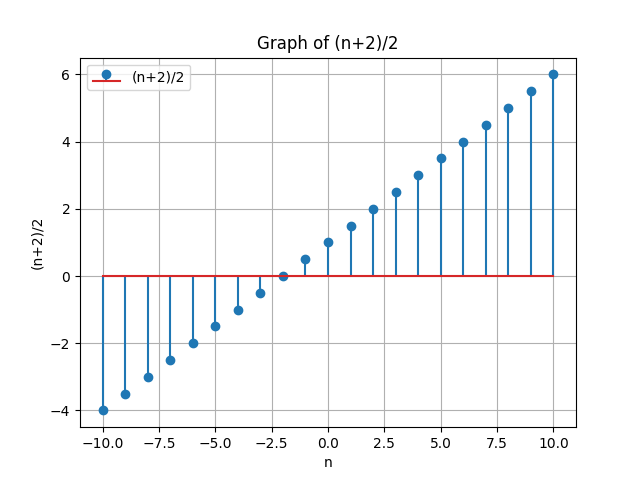
\includegraphics[scale=0.60]{py_3.png}
    \label{fig:enter-label}
\end{figure}

\begin{figure}[h]
    \centering
    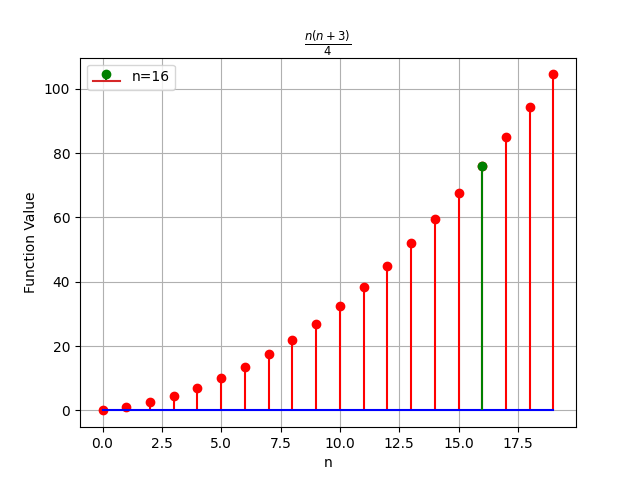
\includegraphics[scale=0.60]{py_4.png}
    \label{fig:enter-label}
\end{figure}

\begin{figure}[h]
    \centering
    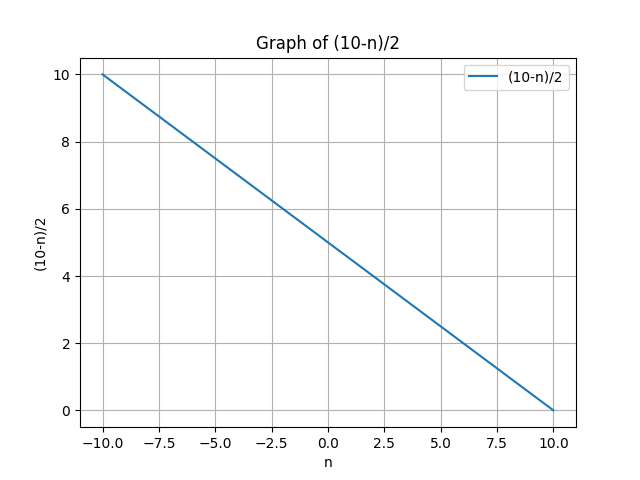
\includegraphics[scale=0.60]{py_5.png}
    \label{fig:enter-label}
\end{figure}

\begin{figure}[h]
    \centering
    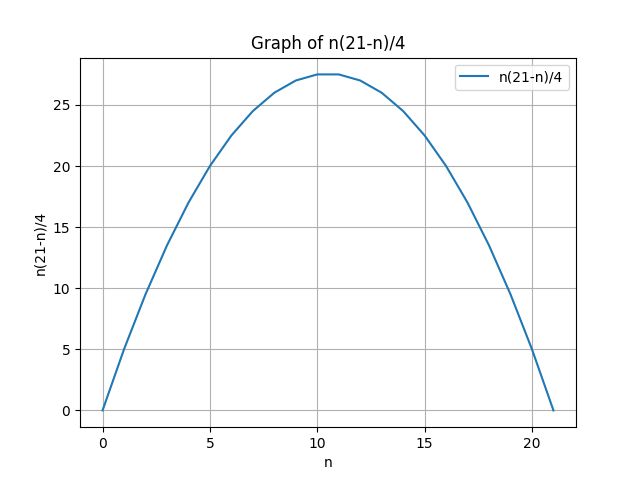
\includegraphics[scale=0.60]{py_6.png}
    \label{fig:enter-label}
\end{figure}
We know that Z-Transform of x\brak{n} is given by:
\begin{align}
\label{q11}
    X\brak{z}=\sum_{k=-\infty}^{\infty} x\brak{k}.z^{-k}
\end{align}
where, we assume that x\brak{k}=0   for \brak{k<0}\\
Then, \brak{\ref{q11}} modifiy as follows:
\begin{align}
\label{q12}
    X\brak{z}=\sum_{k=0}^{\infty} x\brak{k}.z^{-k}
\end{align}
$$X\brak{z}=\sum_{k=0}^{\infty} \brak{\frac{k+2}{2}}.z^{-k}$$
\begin{align}
    \label{q13}
    X\brak{z}=\frac{1}{2}\brak{\sum_{k=0}^{\infty}k.z^{-k}}+\sum_{k=0}^{\infty}z^{-k}
\end{align}
Then consider sum, say S:
$$S=\brak{\sum_{k=0}^{\infty}k.z^{-k}}$$
\begin{align}
\label{q14}
S=0+\frac{1}{z}+\frac{2}{z^2}+\frac{3}{z^3}....\infty
\end{align}
for $Z\neq 0$
\begin{align}
\label{q15}
\frac{S}{z}=0+\frac{1}{z^2}+\frac{2}{z^3}+\frac{3}{z^4}....\infty
\end{align}
Then from \brak{\ref{q15}}-\brak{\ref{q11}}
$$S\brak{1-z^{-1}}=\sum_{k=1}^{\infty}z^{-k}$$
\begin{align}
\label{q16}
    S=\frac{\sum_{k=0}^{\infty}z^{-k}-1}{1-z^{-1}}=\frac{Z}{\brak{Z-1}^2}\ for\ \brak{|Z^{-1}|<1}
\end{align}
So,\brak{\ref{q16}} in \brak{\ref{q13}} Then,
$$X\brak{Z}=\frac{1}{2}\left(\frac{\brak{\sum_{k=0}^{\infty}z^{-k}}-1}{1-z^{-1}}+\sum_{k=0}^{\infty}z^{-k}\right)$$
$$X\brak{Z}=\left(\lim_{n\to\infty}\sum_{k=0}^{n}z^{-k}\brak{\frac{1}{2.\brak{1-z^{-1}}}+1}\right)-\frac{1}{2\brak{1-Z^{-1}}}$$
$$X\brak{Z}=\brak{\frac{1}{2.\brak{1-z^{-1}}}+1}.\left(\lim_{n\to\infty}\sum_{k=0}^{n}z^{-k}\right)-\frac{1}{2\brak{1-Z^{-1}}}$$
$$X\brak{Z}=\brak{\frac{1}{2.\brak{1-z^{-1}}}+1}.\lim_{n\to\infty}\brak{\frac{1-\brak{z^{-1}}^{n+1}}{1-z^{-1}}}-\frac{1}{2\brak{1-Z^{-1}}}$$
So,
$$ X_1\brak{Z}=\frac{2-z^{-1}}{2.\brak{1-z^{-1}}^2}\quad for\ |z^{-1}|<1$$
or,
$$X_1\brak{Z}\ is\ not\ defined\qquad for\ |z^{-1}|>1 $$
From \brak{\ref{q12}},
$$X\brak{Z}=\sum_{k=0}^{\infty} \brak{\frac{10-k}{2}}.z^{-k}$$
$$X\brak{Z}=5.\brak{\sum_{k=0}^{\infty}z^{-k}}-\frac{1}{2}\brak{\sum_{k=0}^{\infty}k.z^{-k}}$$
Then from \brak{\ref{q16}},
$$X\brak{Z}=5.\brak{\sum_{k=0}^{\infty}z^{-k}}-\frac{1}{2}\left(\frac{\sum_{k=0}^{\infty}z^{-k}-1}{1-z^{-1}}\right)$$
$$X\brak{Z}=\left(\brak{5-\frac{1}{2.\brak{1-z^{-1}}}}\lim_{n\to\infty}\sum_{k=0}^{n}z^{-k}\right)+\frac{1}{2\brak{1-Z^{-1}}}$$
$$X_2\brak{Z}=\frac{11.\brak{1-z^{-1}}-1}{2.\brak{1-z^{-1}}^2}\quad for\quad |z^{-1}|<1$$
$$X_2\brak{Z}\ is\ not\ defined\quad for\qquad |z^{-1}|>1$$
\begin{figure}[h]
    \centering
    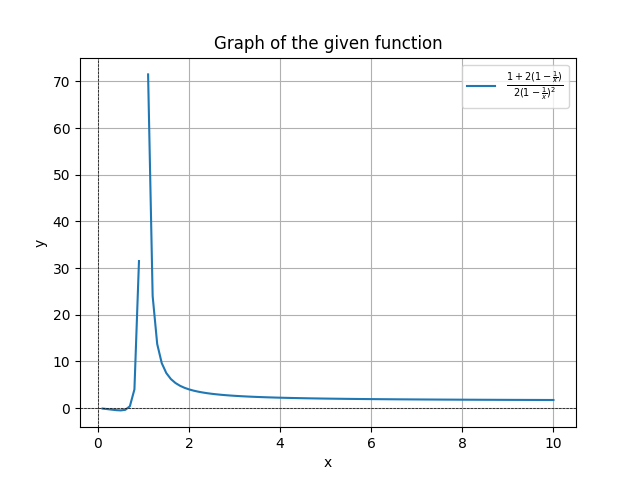
\includegraphics[scale=0.52]{py_31.png}
    \label{fig:enter-label}
\end{figure}\\
\begin{figure}[h]
    \centering
    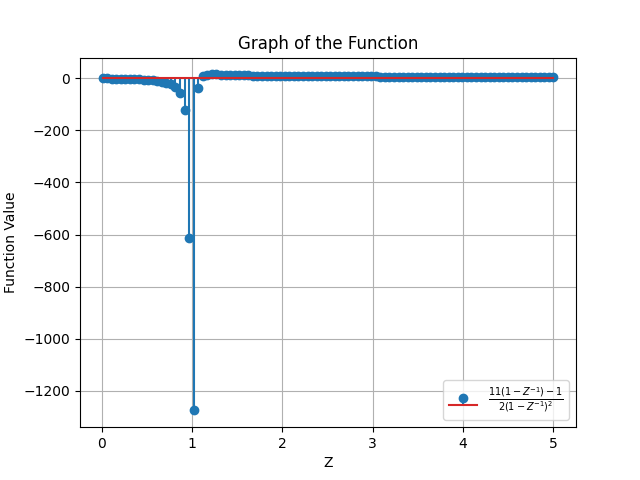
\includegraphics[scale=0.52]{py_32.png}
    \label{fig:enter-label}
\end{figure}\\\\

Let, $\mathcal{Z}$ tranform of s(n) be S(Z):\\
from \brak{\ref{q11}}:
$$S\brak{Z}=\sum_{k=-\infty}^{\infty}s(k)\ Z^{-k}=\sum_{k=0}^{\infty}s(k)\ Z^{-k}\quad \brak{s\brak{k}=0\ for\ k<0}$$
from \brak{\ref{q9}}
$$S\brak{Z}=\sum_{k=-\infty}^{\infty}\left(\brak{x\brak{0}-\frac{d}{2}}k+\frac{d}{2}\ k^2\right).Z^{-k}$$
\begin{align}
\label{q17}
    S\brak{Z}=\brak{x\brak{0}-\frac{d}{2}}\left(\sum_{k=0}^{\infty}k.Z^{-k}\right)+\frac{d}{2}.\left(\sum_{k=0}^{\infty}k^2.Z^{-k}\right)
\end{align}
Let, 
$$
\alpha = \sum_{k=0}^{\infty}k^2.Z^{-k}
$$

\begin{align}
\label{q18}
    \alpha=\frac{1}{Z}+\frac{4}{Z^2}+\frac{9}{Z^3}+\frac{16}{Z^4}+\frac{25}{Z^5}...\infty
\end{align}

\begin{align}
\label{q19}
    \frac{\alpha}{Z}=\frac{1}{Z^2}+\frac{4}{Z^3}+\frac{9}{Z^4}+\frac{16}{Z^5}+\frac{25}{Z^6}...\infty
\end{align}

$\brak{\ref{q17}}$-$\brak{\ref{q18}}$ gives,

\begin{align}
\label{q20}
   \alpha\brak{1-Z^{-1}}=\frac{1}{Z}+\frac{3}{Z^2}+\frac{5}{Z^3}+\frac{7}{Z^4}+\frac{9}{Z^5}...\infty 
\end{align}

\begin{align}
\label{q21}
   \alpha Z^{-1}\brak{1-Z^{-1}}=\frac{1}{Z^2}+\frac{3}{Z^3}+\frac{5}{Z^4}+\frac{7}{Z^5}+\frac{9}{Z^6}...\infty 
\end{align}

$\brak{\ref{q19}}$-$\brak{\ref{q20}}$ gives,

$$\alpha\brak{1-Z^{-1}}^2=\frac{1}{Z}+\frac{2}{Z^2}+\frac{2}{Z^3}+\frac{2}{Z^4}+\frac{2}{Z^5}+...\infty$$

$$\alpha\brak{1-Z^{-1}}^2=\frac{1}{Z}+\frac{2}{Z^2}\left(1+\frac{1}{Z}+\frac{1}{Z^2}+\frac{1}{Z^3}...\infty\right)$$

$$\alpha\brak{1-Z^{-1}}^2=\frac{1}{Z}+\frac{2}{Z^2}\left(\sum_{k=0}^{\infty}Z^{-k}\right)$$

$$
\alpha=\brak{1-Z^{-1}}^{-2}.\left(\frac{1}{Z}+\frac{2}{Z^2}\left(\sum_{k=0}^{\infty}Z^{-k}\right)\right)
$$

$$
\alpha=\brak{1-Z^{-1}}^{-2}.\left(\frac{1}{Z}+\frac{2}{Z^2}\lim_{n\to\infty}\brak{\frac{1-\brak{z^{-1}}^{n+1}}{1-z^{-1}}}\right)
$$
$$
\alpha=\brak{1-Z^{-1}}^{-2}.\left(\frac{1}{Z}+\frac{2}{Z^2}\brak{\frac{1}{1-z^{-1}}}\right)\quad for\ |Z^{-1}|<1
$$
$$\alpha=\brak{1-Z^{-1}}^{-2}.\left(\frac{1}{Z}\right)\left(\frac{Z+1}{Z-1}\right)
$$

\begin{align}
\label{q22}
\alpha=\frac{Z\brak{Z+1}}{\brak{Z-1}^3}
\end{align}

from \brak{\ref{q16}} and \brak{\ref{q22}} in \brak{\ref{q17}}

$$
S\brak{Z}=\brak{x\brak{0}-\frac{d}{2}} S+\frac{d}{2}\ \alpha
$$

$$
S\brak{Z}=\brak{x\brak{0}-\frac{d}{2}}\frac{Z}{\brak{Z-1}^2}+\frac{d}{2}\left(\frac{Z\brak{Z+1}}{\brak{Z-1}^3}\right)
$$
$$s\brak{Z}=x\brak{0}\left(\frac{Z}{\brak{Z-1}^2}\right)-\frac{d}{2}\left(\frac{Z}{\brak{Z-1}^2}-\frac{Z(Z+1)}{\brak{Z-1}^3}\right)$$

$$s\brak{Z}=x\brak{0}\left(\frac{Z}{\brak{Z-1}^2}\right)+d\left(\frac{Z}{\brak{Z-1}^3}\right)$$

\begin{align}
\label{q23}
S\brak{Z}=\frac{x\brak{0}.Z.\brak{Z-1}+d.Z}{\brak{Z-1}^3}\ for\ |Z^{-1}|<1\ and\ Z\neq0
\end{align}

from \brak{\ref{q23}}, for x\brak{0}=1 and $d=\frac{1}{2}$

$$S\brak{Z}=\frac{Z\brak{Z-\frac{1}{2}}}{\brak{Z-1}^3}$$

\begin{figure}[h]
    \centering
    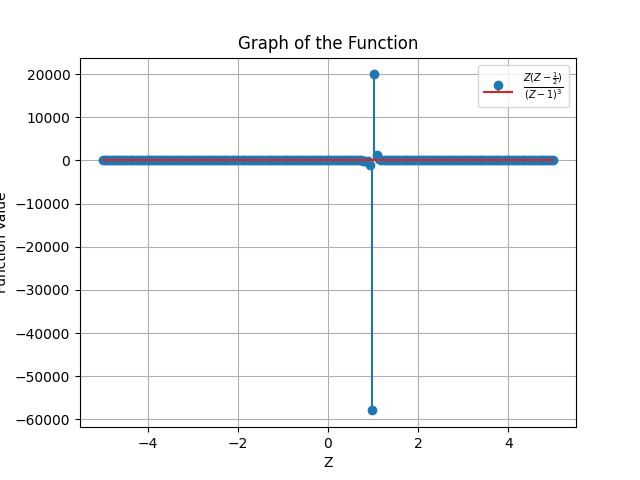
\includegraphics[scale=0.52]{py_33.png}
    \label{fig:enter-label}
\end{figure}

and from \brak{\ref{q23}}, for x\brak{0}=5 and $d=-\frac{1}{2}$

$$S\brak{Z}=\frac{Z\brak{5.Z-\frac{11}{2}}}{\brak{Z-1}^3}$$

\begin{figure}[h]
    \centering
    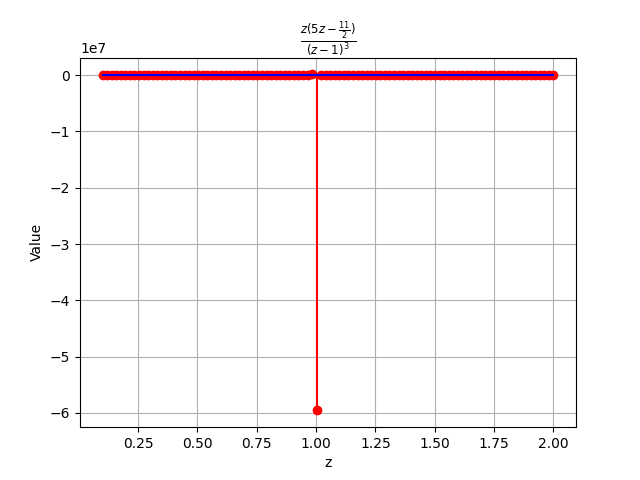
\includegraphics[scale=0.52]{py_34.png}
    \label{fig:enter-label}
\end{figure}

\end{document}
